\subsection*{\lr{2.7.2} اثبات کامل بودن \lr{(Completeness)}}
  
  \begin{theorem}
    اگر فرمول \(A\) نارضایت‌پذیر باشد، آنگاه هر جدولی (tableau) که برای \(A\) ساخته شود، بسته می‌شود.
  \end{theorem}
  
  برای اثبات، به‌جای مستقیم نشان می‌دهیم:
  
  \begin{corollary}[نتیجه گیری \lr{2.68}]
    اگر جدولی برای \(A\) باز باشد (یعنی دارای حداقل یک شاخهٔ باز)، آنگاه \(A\) برآورده‌پذیر (satisfiable) است.
  \end{corollary}
  
  روش کار در چهار گام اصلی است:
  \begin{enumerate}[1)]
    \item تعریف مجموعهٔ هینتیکا \lr{(Hintikka set)}.
    \item اثبات اینکه اجتماع برچسب‌های گره‌های یک شاخهٔ باز، یک مجموعهٔ هینتیکا است.
    \item اثبات اینکه هر مجموعهٔ هینتیکا برآورده‌پذیر است.
    \item نشان دادن اینکه خود فرمول \(A\) (برچسب ریشه) در آن مجموعه حضور دارد.
  \end{enumerate}
  
  \begin{definition}[مجموعهٔ هینتیکا]\label{def:2.75}
  مجموعه‌ای از فرمول‌ها را \emph{مجموعهٔ هینتیکا} می‌نامیم اگر:
  \begin{enumerate}[1)]
    \item برای هر اتم \(p\) که در مجموعه هست، دقیقاً یکی از \(p\in U\) یا \(\neg p\in U\) برقرار باشد.
    \item اگر \(A\in U\) یک فرمول \(\alpha\) باشد (یعنی \(A=A_1\land A_2\))، آنگاه \(A_1, A_2\in U\).
    \item اگر \(B\in U\) یک فرمول \(\beta\) باشد (یعنی \(B=B_1\lor B_2\))، آنگاه \(B_1\in U\) یا \(B_2\in U\).
  \end{enumerate}
  \end{definition}
  
  \begin{example}[مثال \lr{2.73}]
  فرض کنید
  \[
    A = p \land (\neg q \lor \neg p).
  \]
  یک جدول ممکن:
  \begin{center}
    \begin{latin}
      \resizebox{0.35\textwidth}{!}{
      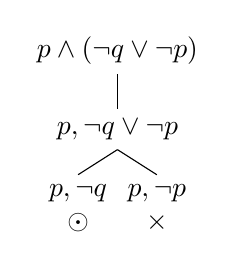
\begin{tikzpicture}[
        level distance=1cm,
        sibling distance=1.5cm,
        level 2/.style={sibling distance=1cm},
        edge from parent path={(\tikzparentnode.south) -- (\tikzchildnode.north)}
      ]
      \node {$p \land (\neg q \lor \neg p)$}
        child { 
          node {$p, \neg q \lor \neg p$}
          child { node[align=center] {$p, \neg q$ \\ $\odot$} }
          child { node[align=center] {$p, \neg p$ \\ $\times$} }
        };
      \end{tikzpicture}
      }  
    \end{latin}
  \end{center}
  شاخهٔ \(p,\neg q\) باز است با \(p=T,\,q=F\) که مدلی برای \(A\) می‌سازد.
  \end{example}
  
  \begin{example}[مثال \lr{2.74}]
  فرض کنید
  \[
    A = p \lor (q\land\neg q).
  \]
  یک جدول ممکن:
  \begin{center}
    \begin{latin}
      \resizebox{0.35\textwidth}{!}{
      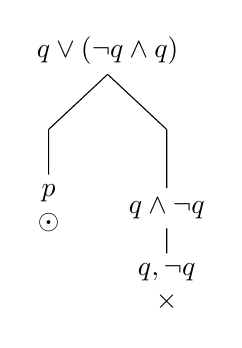
\begin{tikzpicture}[
        level distance=1cm,
        sibling distance=1.5cm,
        level 2/.style={sibling distance=1cm},
        edge from parent path={(\tikzparentnode.south) -- (\tikzchildnode.north)}
      ]
      \node {$q \lor (\neg q \land q)$}
        child { 
          child { node[align=center] {$p$ \\ $\odot$} }
        }
        child { 
          child { 
            node {$q \land \neg q$}
            child { node[align=center] {$q, \neg q$ \\ $\times$} }
          }
        };
      \end{tikzpicture}
      }  
    \end{latin}
  \end{center}
  شاخهٔ \(p\) باز است، پس هر مدلی باید \(p=T\) باشد.
  \end{example}
  
  \begin{theorem}[قضیهٔ \lr{2.77}]
  اگر \(l\) یک برگ باز در جدول تکمیل‌شده \(T\) باشد، آنگاه
  \[
    U \;=\;\bigcup_{i\in\text{شاخه از ریشه تا }l} U(i)
  \]
  یک مجموعهٔ هینتیکا است.
  \end{theorem}
  \begin{proof}
  \begin{enumerate}[1)]
    \item لیترال‌ها در هیچ قاعده‌ای شکسته نمی‌شوند و از ریشه تا برگ منتقل می‌گردند. چون برگ باز است، جفت متضاد در \(U(l)\) نیست، پس شرط (1) برقرار است.
    \item اگر \(A\in U\) یک \(\alpha\)-فرمول باشد، در مسیر تجزیه شده و زیرفرمول‌های \(A_1,A_2\) در \(U\) قرار می‌گیرند.
    \item اگر \(B\in U\) یک \(\beta\)-فرمول باشد، در مسیر تجزیه شده و یکی از زیرفرمول‌های \(B_1\) یا \(B_2\) در \(U\) قرار می‌گیرد.
  \end{enumerate}
  بنابراین \(U\) هینتیکا است.
  \end{proof}
  
  \begin{theorem}[لم هینتیکا \lr{2.78}]
  اگر \(U\) یک مجموعهٔ هینتیکا باشد، آنگاه \(U\) برآورده‌پذیر است.
  \end{theorem}
  \begin{proof}
  اتم‌های \(P_U\) را مجموعهٔ اتم‌های ظاهرشده در \(U\) در نظر بگیرید. تفسیر
  \(\mathscr{I}\) را تعریف می‌کنیم:
  \[
  \mathscr{I}(p)=
  \begin{cases}
  \mathsf{T}, & p\in U,\\
  \mathsf{F}, & \neg p\in U,\\
  \mathsf{T}, & \text{اگر }p,\neg p\notin U.
  \end{cases}
  \]
  شرط (1) تناقض را نفی می‌کند. سپس با استقرا بر ساختار فرمول‌ها نشان می‌دهیم برای هر \(A\in U\)، \(v_{\mathscr{I}}(A)=\mathsf{T}\):
  \begin{itemize}
    \item اگر \(A=p\) یا \(A=\neg p\)، واضح است.
    \item اگر \(A=A_1\land A_2\)، شرط (2) هر دو \(A_1,A_2\in U\) را تضمین می‌کند.
    \item اگر \(A=B_1\lor B_2\)، شرط (3) یکی از آنها را تضمین می‌کند.
  \end{itemize}
  پس \(\mathscr{I}\) مدلی از \(U\) است.
  \end{proof}
  
  \subsubsection*{نتیجه‌گیری}
  اگر \(T\) جدولی باز و تکمیل‌شده برای \(A\) باشد، اجتماع برچسب‌های شاخهٔ باز مجموعه‌ای هینتیکا می‌سازد (قضیهٔ \lr{2.77}) و از لم هینتیکا (قضیهٔ \lr{2.78}) این مجموعه مدل دارد. چون \(A\) در برچسب ریشه هست، \(\mathscr{I}\) مدلی برای \(A\) می‌شود و بنابراین اثبات کامل بودن پایان می‌یابد.